\chapter{Grundlagen\label{chap2:Zweites-Kapitel}}

Um eine Konzeption und eine prototypische Umsetzung einer Search Engine in \gls{mcc} zu ermöglichen wird in folgendem Kapitel auf die architekturellen Hintergründe von \gls{mcc} eingegangen. Hierfür werden zu Beginn allgemein gültige Architektur-Prinzipien erläutert, welche auch bei der Integration einer Search Engine berücksichtigt werden müssen und somit bei der Auswahl eines geeigneten Konzeptes von Bedeutung sind.

Aufbauend auf den Architektur-Prinzipien wird die verwendete Microservice-Architektur erläutert, wobei neben einer allgemeinen Einführung in die Architektur auch auf die Kommunikation von Microservices untereinander eingegangen wird. Um mögliche Fehlkonzeptionen zu vermeiden, werden häufig auftretende Anti-Pattern aufgezeigt, welche unter Umständen zu monolithischen Seiteneffekten führen könnten.

Abschließend wird anhand von verschiedenen modernen Informationssystemen die Funktionalitäten der Volltextsuche gezeigt. Neben den unterschiedlichsten Anwendungsfällen für eine Volltextsuche werden auch die technischen Besonderheiten von Search Engines vorgestellt.

\section{Software-Architekturen\label{sec2.1:Unterpunkt-1}}

\begin{quote}
    Die Software-Architektur eines Systems ist die Menge von Strukturen, die benötigt werden, um Entscheidungen über das System zu treffen, welche die Software-Elemente, die Relationen zwischen ihnen und die Eigenschaften von beiden betreffen. \textasciitilde{} Len Bass \cite{Bass.2013}
\end{quote}

Wie aus der Definition von Len Bass zu entnehmen ist, beschreibt eine Software-Architektur die Eigenschaften und Beziehungen von Software-Bausteinen zueinander \cite{Bass.2013}. Ein Software-Baustein wird hierbei als eine Teil-Komponente der gesamten Software betrachtet und wird bei der Erstellung einer Architektur als elementarer Bestandteil angesehen. Dabei wird ein Software-Baustein nicht näher spezifiziert, sondern als Komponente betrachtet, dessen konkrete Implementierung für die Architektur nicht von Bedeutung ist. Der Fokus einer Software-Architektur liegt auf den Schnittstellen der Software-Bausteine, über welche die Bausteine miteinander kommunizieren können.

\subsection{Architektur-Prinzipien\label{subsec2.1.1:Unterunterpunkt-1}}

Für das Erstellen einer guten Software-Architektur wurden von Vogel \cite{Vogel.2009} einige Grundprinzipien definiert. Diese Prinzipien sollten bei der Erstellung einer Software-Architektur beachtet werden: \cite{Vogel.2009}

\begin{description}
    \item[Lose Kopplung:]\hfill \\
    Der Kern einer Software-Architektur besteht aus der Beschreibung der Bausteine eines Software-Systems und deren Interaktionen zueinander. Unter dem Begriff Kopplung versteht man hierbei die Beziehung unter den Bausteinen einer Software-Architektur. Eine Kopplung charakterisiert demnach die Interaktionen der Bausteine.

    Eine starke Kopplung von Systembausteinen hat zur Folge, dass beim Verstehen und Ändern eines Bausteines auch zwingend weitere Bausteine verstanden und geändert werden müssen. Um jenes Problem zu umgehen, besagt das Prinzip der losen Kopplung, dass die Kopplung zwischen Systembausteinen möglichst niedrig gehalten werden sollen.

    Um eine lose Kopplung in einer Architektur zu erreichen, ist die Einführung von Schnittstellenabstraktionen ein wichtiger Aspekt. Dabei werden die Implementierungsinformationen hinter den Schnittstellen verborgen. Durch die Begrenzung von Schnittstellenelementen und der Häufigkeit des Austauschs der Schnittstellenelemente kann eine Kopplung von Systembausteinen kontrollierbar gemacht werden.

    \item[Hohe Kohäsion:]\hfill \\
    Im Gegensatz zur Kopplung, in welcher die Beziehungen zwischen Systembausteinen gemeint ist, versteht man unter dem Begriff Kohäsion die Abhängigkeiten innerhalb eines Systembausteins.

    Beim Prinzip der hohen Kohäsion ist das Ziel die Abhängigkeiten innerhalb eines Systembausteins möglichst hoch zu gestalten. Wie bei der losen Kopplung geht es auch hier um die lokale Änderbarkeit und Verstehbarkeit von Systembausteinen.
    
    Wie in \autoref{fig:kopplung_and_kohaesion} zu erkenne stehen Kopplung und Kohäsion normalerweise miteinander in einer Wechselbeziehung. Hierbei gilt, dass je höher die Kohäsion individueller Bausteine einer Architektur ist, desto geringer ist die Kopplung zwischen den Bausteinen. Schematisch ist dieser Zusammenhang in \autoref{fig:kopplung_and_kohaesion} abgebildet, worin zu erkennen ist, das eine Gesamtstruktur mit einer hohen Kohäsion und einer losen Kopplung (rechte Seite) eine höhere Übersichtlichkeit besitzt.

    \begin{figure}[H]
        \centering
        \includegraphics[width=0.7\linewidth]{images/Kopplung_und_Kohäsion.png}
        \caption{Zusammenspiel von loser Kopplung und hoher Kohäsion \cite{Vogel.2009}}
        \label{fig:kopplung_and_kohaesion}
    \end{figure}

    \item[Entwurf für Veränderung:]\hfill \\
    Durch den stetigen Wandel von Software-Systemen in Form von Anforderungen und Technologien, ist es von Vorteil solche Änderungen bereits in der Phase der architekturellen Konzeption zu berücksichtigen. Das Prinzip des Entwurfs für Veränderung (englisch: Design for Change) sieht nun vor, dass man vorhersehbare Änderungen architektonisch vorausplant. Dabei sollte man versuchen, die Architektur so zu entwerfen, dass man leicht mit den wahrscheinlichen Änderungen eines Software-Systems umgehen kann.

    \item[Separation of Concerns:]\hfill \\
    Abgeleitet von dem römischen Prinzip \glqq Teile und herrsche\grqq{} wird beim Prinzip Separation of Concerns ausgesagt, dass ein Software-System in individuelle Systembausteine zerlegt werden soll.

    Separation of Concerns unterstützt hierbei die Modularisierung eines Software-Systems. Es geht darum Teile eines Software-Systems zu identifizieren, welche für bestimmte Angelegenheiten, Aspekte und Aufgaben verantwortlich sind. Jene Teile werden dann als eigene Systembausteine gekapselt. Eine Zerteilung des Gesamtsystems in relativ unabhängige Einzelteile ermöglicht zudem noch die Verteilung von Verantwortlichkeiten für verschiedene Systembausteine und auch das parallele Arbeiten an dem Software-System durch mehrere Entwickler wird dadurch ermöglicht.

    Durch das Aufteilen des Software-Systems in relativ unabhängige Systembausteine werden auch die Prinzipien lose Kopplung und hohe Kohäsion begünstigt.

    \item[Information Hiding:]\hfill \\
    Das Prinzip Information Hiding sagt aus, dass man einem Klienten nur die für die Bearbeitung eines Problems notwendigen Informationen zeigen soll. Dies erleichtert die Gliederung und das Verständnis von komplexen Software-Systemen. Die restlichen Informationen sollen nach außen hin verborgen bleiben. Ermöglicht wird solch ein geheim halten von Informationen durch die Bereitstellung von definierten Schnittstellen, über welche nur bestimmte Informationen zu erreichen sind.

    \item[Abstraktion:]\hfill \\
    Als übergeordnetes Prinzip dient eine Abstraktion dazu, ein komplexes System verständlicher zu machen. Dazu werden wichtige Aspekte identifiziert und unwichtige Details vernachlässigt. Im Bereich der Software-Architektur gilt die Schnittstellenabstraktion als Teilprinzip der Abstraktion. Hierbei liegen die Schnittstellen im Fokus, welche für das Zustandekommen und die Qualität von Beziehungen verantwortlich sind.

    Solch eine Schnittstellenabstraktion in einem Software-System ist eng verbunden mit dem Prinzip der losen Kopplung und dem Information Hiding. Ein Aspekt für den starken Zusammenhang zwischen der Abstraktion und dem Information Hiding ist die Portabilität von Software-Systemen. So sollte eine Architektur oder ihre Systembausteine auch in anderen Umgebungen verwendbar sein. Um solch eine Plattformunabhängigkeit sicherzustellen, werden Abstraktionen verwendet, die ein Information Hiding der Platform-Details leisten.

    \item[Modularität:]\hfill \\
    Das Modularitätsprinzip, welches bereits auch in den Beschreibungen der anderen Prinzipien vorkam, definiert die Aufteilung eines Systems in klar definierte Bausteine mit abgegrenzten funktionalen Verantwortlichkeiten. Die Modularität ist dabei eine Kombination aus den Prinzipien Abstraktion, Separation of Concerns und Information Hiding, welche bei der Umsetzung der Prinzipien der losen Kopplung und der hohen Kohäsion kombiniert werden.

\end{description}

Auch für die spätere Konzeption einer Search Engine in einer Microservice-Architektur werden die eingeführten Prinzipien als Grundlage dienen.

\subsection{Monolithische und verteilte Architekturen\label{subsec2.1.2:Unterunterpunkt-2}}

Bei der Neugestaltung von E-MES wird von einer monolithischen 3-Schichten-Architektur auf eine verteilte Microservice-Architektur gewechselt.

Dabei besaß die ehemalige E-MES Architektur eine monolithische Struktur. In einer solchen monolithische Architektur wird die gesamte Architektur in nur einem Systembaustein zusammengefasst. Dadurch erfolgt keine explizite Gliederung in Teilsysteme und Architektur-Prinzipien, wie lose Kopplung und Separation of Concerns sind nur schwer umsetzbar \cite{Vogel.2009}. Zu finden sind monolithische Architekturen oftmals in Altsystemen, welche oft über Jahrzehnte gewachsen sind. Aufgrund der mangelnden Modularisierung steigt die Kompliziertheit des Systems und eine Wartung und Anpassung des Quellcodes wird erschwert \cite{Prof.Dr.AndreasFink.2012b}. Ein weiterer Nachteil der mangelnden Modularisierung ist die kaum mögliche nebenläufige Ausführung von Teilen des Systems auf verschiedenen Rechnern \cite{Prof.Dr.AndreasFink.2012b}. Somit kann eine horizontale Skalierung nicht ermöglicht werden und eine effiziente, lastverteilende Programmausführung ist nicht gegeben.

Die Architektur von MCC wird eine verteilte Struktur aufweisen. Hierbei werden Teile des Gesamtsystems in unterschiedliche Systembausteine aufgeteilt. Eine Modularisierung der Software ist dadurch möglich und Architekturen-Prinzipien, wie lose Kopplung und Separation of Concerns sind umsetzbar \cite{Vogel.2009}. Durch die strikte Aufteilung der Geschäftslogik kann auch die Komplexität aufgeteilt werden. Somit können die einzelnen Systembausteine mit wenig Aufwand angepasst oder erweitert werden. Durch die Modularisierung von verteilten Architektur kann die Ausführung bestimmter Aufgaben auf redundanter Hardware nebenläufig erfolgen \cite{Prof.Dr.AndreasFink.2012}. Durch jene horizontale Skalierung kann eine effiziente und lastverteilende Programmausführung erfolgen, welche auch zur Ausfallsicherheit des Gesamtsystems beiträgt \cite{Prof.Dr.AndreasFink.2012}.

% \begin{figure}[H]
%     \centering
%     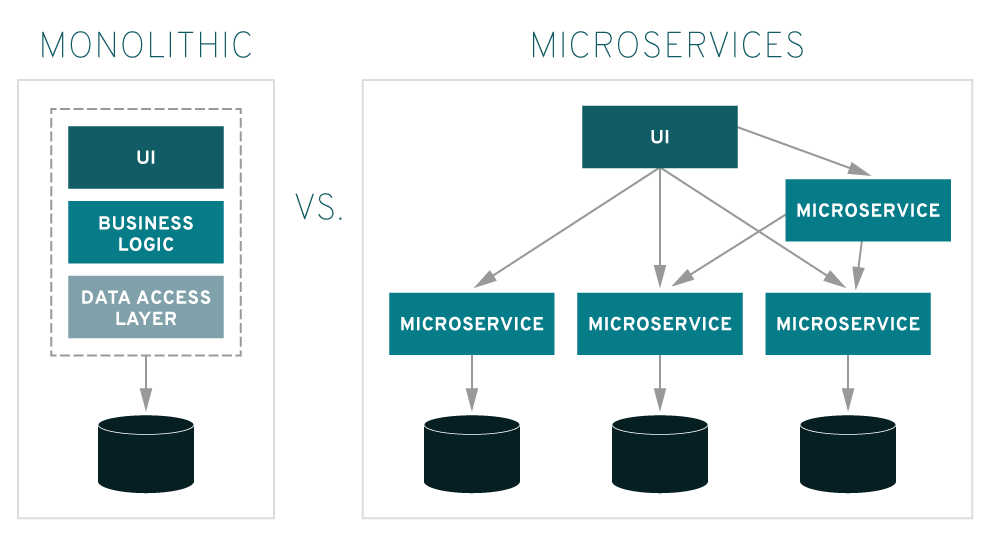
\includegraphics[width=0.7\linewidth]{images/monolithic-vs-microservices.png}
%     \caption{3-Schichten-Architektur vs. Microservice-Architektur \cite{RedHatLimited.2021}}
%     \label{fig:mono_vs_micro}
% \end{figure}

\section{Microservice-Architektur\label{sec2.2:Unterpunkt-2}}

Als eine Architektur mit einer verteilten Struktur, wird die Software bei der Neugestaltung des \gls{mes} der Firma Enisco, auf einer Microservice-Architektur aufgebaut.

Die Kernelemente dieser Architektur sind die Microservices, welche der Modularisierung der Software dienen. Somit ist eine Aufteilung des Gesamtsystems in verschiedene Systembausteine möglich. Ein Systembaustein stellt dabei jeweils eine Funktionalität des Gesamtsystems dar. Im Gegensatz zu einer monolithischen Architektur läuft das Gesamtsystem nicht innerhalb eines Prozesses, sondern auf verschiedenen Prozessen. Dabei wird jedem Systembaustein ein eigener Prozess zugeordnet. Jene Prozesse können nun nahezu beliebig auf verschiedene Rechner verteilt und durch Replizierung ausfallsicher gemacht werden. \cite{GaryCalcott.2018}

Neben den Vorteilen der horizontalen Skalierung, ergeben sich aus der Aufteilung des Gesamtsystems in unterschiedliche Systembausteine auch Auswirkungen auf die Entwicklungsorganisation. So wird beim Umgang mit Microservices nach der Unix-Philosophie von Ken Thompson \glqq Do one thing and do ot well\grqq{} \cite{IONOSSE.2021} gearbeitet. Durch die Modularität von Microservices untereinander können die Microservices von unterschiedlichen Entwicklerteams unabhängig voneinander entwickelt werden. Durch die Abstraktion der Microservices, können diese mit unterschiedlichen Technologien und Programmiersprachen implementiert werden. Auch der Datenhaushalt kann von jedem Microservice separat verwaltet werden. Zudem wird die Einarbeitung eines Entwicklers in die Codebasis reduziert, da durch die Aufteilung weniger Code verstanden werden muss.

Die Microservice-Architektur berücksichtigt die Architektur-Prinzipien Separation of Concerns, Information Hiding und Modularität und gewährleisten somit eine lose Kopplung zwischen den Microservices. Innerhalb der Microservices entsteht dadurch eine hohe Kohäsion.

Da die jeweiligen Microservices repliziert auf verschiedenen Rechnern laufen können, ist die Kommunikation zwischen den Microservices schwieriger als bei einem monolithischen System. Auf die Kommunikation zwischen Microservices wird in \autoref{subsec2.2.1:Unterunterpunkt-1} näher eingegangen.

Eine Herausforderung bei der Entwicklung einer Microservice-Architektur ist die Vermeidung von Abhängigkeiten, welche eine lose Kopplung der Microservices verhindern. Um solche monolithischen Seiteneffekten zu vermeiden, werden in \autoref{subsec2.2.2:Unterunterpunkt-2} die häufigsten Microservice-Antipattern aufgezeigt.

\subsection{Kommunikation zwischen Microservices\label{subsec2.2.1:Unterunterpunkt-1}}

Auch wenn das Ziel einer Microservice-Architektur ist, dass einzelne Funktionalitäten des Gesamtsystems in getrennte Microservices gekapselt werden, müssen jene miteinander kommunizieren. Aufgrund der Modularität können die Microservices horizontal skaliert werden und auf verschiedenen Rechnern betrieben werden. Dies erhöht die Komplexität bei der Kommunikation der Microservices untereinander. \cite{MichaelSchwab.2019}

Bei der Wahl der Kommunikation zwischen Microservices kann zwischen einer synchronen und asynchronen Kommunikation entschieden werden.

\subsubsection*{Synchrone Kommunikation}

Bei der synchronen Kommunikation handelt es sich um eine eins-zu-eins Kommunikation, bei der eine Anfrage geschickt und auf eine Antwort gewartet wird. Klassischerweise erfolgt die Kommunikation über HTTP mit einer REST-Schnittstelle. \gls{rest} ist hierbei eine Spezifikation, wie eine über HTTP kommunizierende API konzipiert werden soll \cite{MichaelSchwab.2019}. Eine solche API sollte demnach vordefinierte HTTP-Methoden implementiert haben. Unter anderem sind das Methoden wie GET, POST, PUT und DELETE. Bei einer GET-Anfrage werden hierbei Ressourcen angefragt. Möchte man einen neuen Datensatz übermitteln wird die POST-Methode verwendet und wenn man einen bestehenden Datensatz ändern möchte, verwendet man die PUT-Methode. Mit der DELETE-Methode kann man einen expliziten Datensatz löschen. Jeder Datensatz bekommt hierbei einen eigenen Endpunkt und die jeweiligen Anfragen können mit URL-Parametern und Query-Parametern spezifiziert werden. Das Standard-Datenformat bei REST ist JSON.

Bei der Kommunikation von zwei Microservices über die jeweiligen REST-Schnittstellen, muss die Adresse des anderen Microservice bekannt sein. Durch die Verteilung der Microservices auf unterschiedliche Rechner in Folge einer horizontalen Skalierung kann es während dem Betrieb vorkommen, dass einzelne Microservices auf zum Beispiel Rechner A gestoppt und auf Rechner B wieder gestartet werden. Dadurch ändern sich auch die Adressen der Microservices. Da die Verwaltung der Adressen ab einer Vielzahl an Microservices nicht mehr trivial ist, wird in einer Microservice-Architektur eine sogenannte Service-Discovery eingesetzt. Die Service-Discovery ist eine Software, bei der sich alle neuen Microservice registrieren. Bei einem REST-Aufruf wird dann zuerst eine Liste mit allen verfügbaren Adressen abgerufen.

Wie in \autoref{fig:service_discovery} zu abgebildet ist, wird bei einer Anfrage eines Services, jene Anfrage zunächst an einen Router-Service geleitet. Nach dem Abfragen der Adresse mithilfe der Service-Discovery wird gezielt der entsprechende Service mit einer REST-Anfrage angesprochen.

\begin{figure}[H]
    \centering
    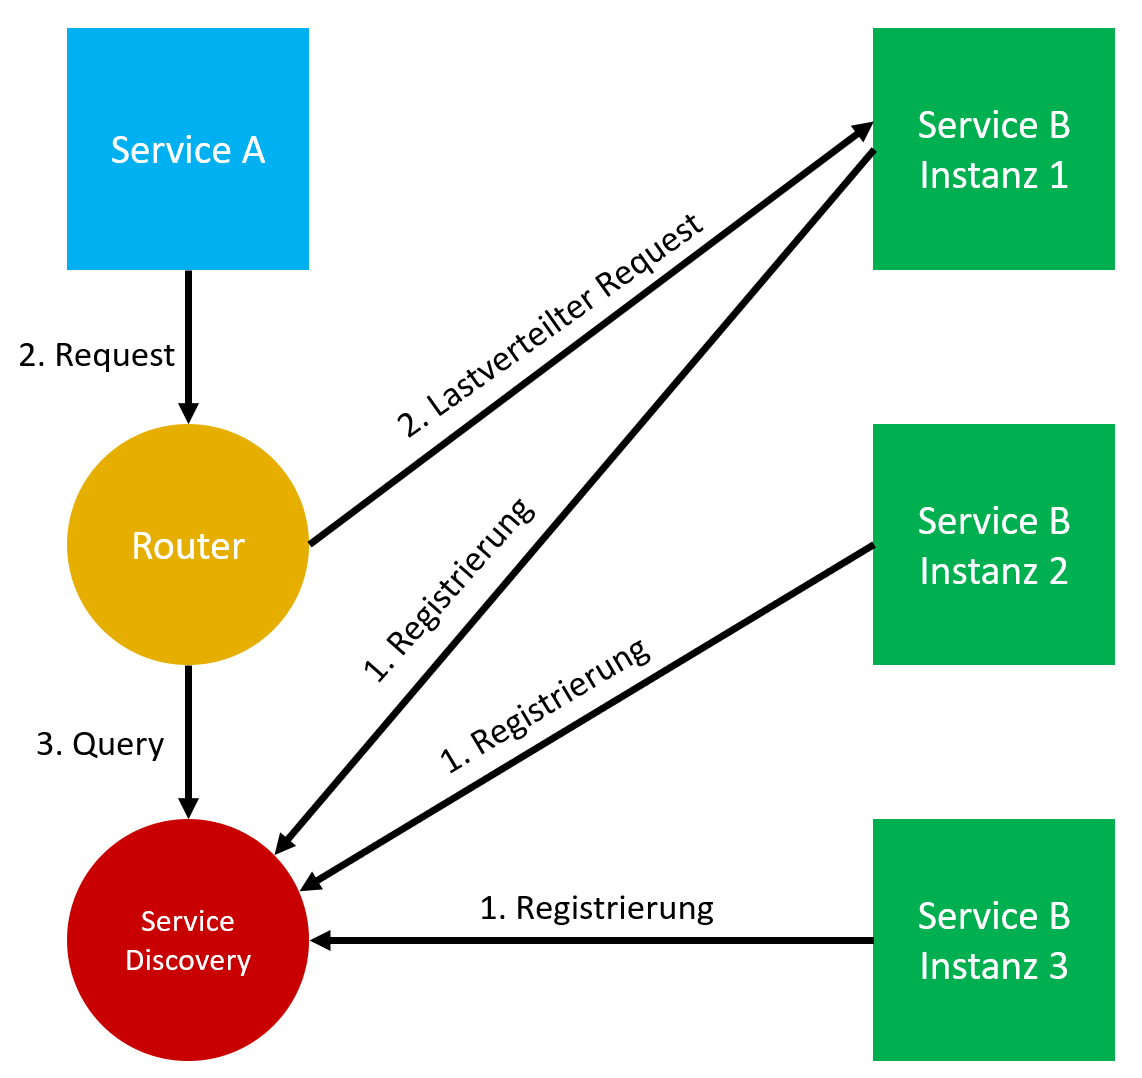
\includegraphics[width=0.65\linewidth]{images/service-discovery.png}
    \caption{Ablauf einer Anfrage mit der Service-Discovery - in Anlehnung an \cite{MichaelSchwab.2019}}
    \label{fig:service_discovery}
\end{figure}

\subsubsection*{Asynchrone Kommunikation}

\subsection{Microservice - Antipattern\label{subsec2.2.2:Unterunterpunkt-2}}

Inhalt

\section{Volltextsuche in modernen Informationssystemen\label{sec2.3:Unterpunkt-3}}

Inhalt

\subsection{Anwendungsfälle\label{subsec2.3.1:Unterunterpunkt-1}}

Inhalt

\subsection{Search Engines\label{subsec2.3.2:Unterunterpunkt-2}}

Inhalt